\documentclass[aspectratio=199]{beamer}
\usetheme{UWMadison}
\usepackage{conference_talk}

\title[BART Introduction]{Applied modeling with BART: \\ How, Why, and When}
\author[S.K. Deshpande]{Sameer K. Deshpande}
\institute[UW--Madison]{University of Wisconsin--Madison}
\date[18 May 2024]{18 May 2024}

\def\nx{\texttt{nx}}

\begin{document}

\begin{frame}[noframenumbering]
\titlepage
\end{frame}

\section{Motivations}
\begin{frame}[noframenumbering]{Overview}
\tableofcontents
\end{frame}

\begin{frame}{Catch probability \& QB rankings}
\begin{itemize}
\item{Which QB's throw the ``most catchable'' balls?}
\item{If we knew $\P(\texttt{catch})$ exactly, we could rank QB's based on}
\begin{itemize}
\item{Avg. $\P(\texttt{catch})$}
\item{Prop.\ of time $\P(\texttt{catch})$ exceeds a threshold (e.g., 80\%)}
\item{Prop.\ of time QB threw to target w/ highest $\P(\texttt{catch})$ on play (EHCP)}
\end{itemize}
\end{itemize}

\visible<2->{
\begin{columns}
\begin{column}{0.54\textwidth}
\begin{itemize}
\item{$\P(\texttt{catch}) = F(\bx_{c}, \bx_{r}, \bx_{a})$}
\item[\Annoey]{$F$ is highly non-linear}
\item[\Annoey]{$F$ may involve complex interactions}
\end{itemize}
\end{column}

\begin{column}{0.45\textwidth}
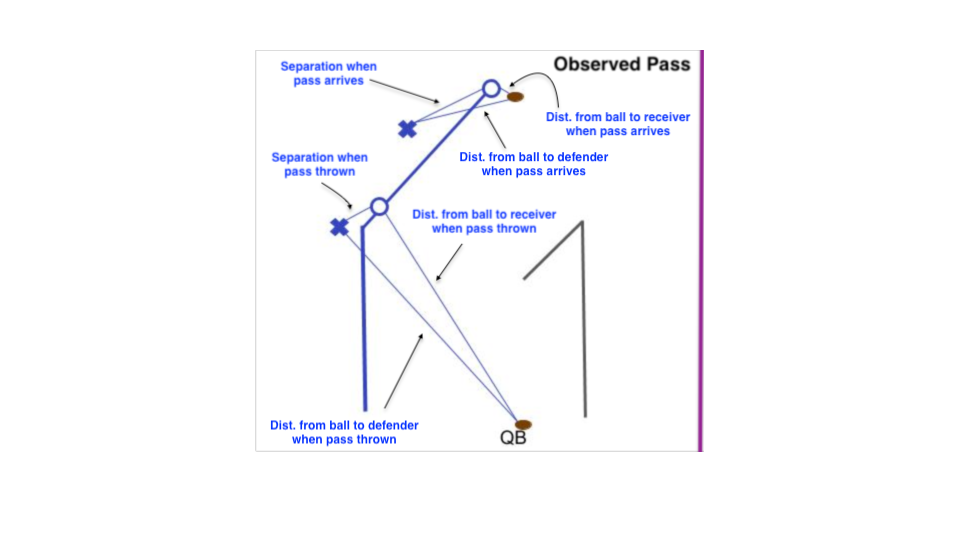
\includegraphics[width = 1.2\textwidth]{figures/observed_route}
\end{column}
\end{columns}
}

\visible<3->{
\begin{itemize}
\item{Uncertainty about $F$ \textbf{propagates} to uncertainty in QB rankings!}
\end{itemize}
}
\end{frame}

\begin{frame}{A more general problem: nonparametric regression}

\begin{itemize}
\item{Observe $(\bx_{1}, y_{1}), \ldots, (\bx_{n}, y_{n})$ and model}
$$
y_{n} = f(\bx_{n}) + \sigma \epsilon_{n}; \epsilon_{n} \sim \normaldist{0}{1}
$$
\item{We have the following goals:}
\begin{itemize}
\item{Prediction: value of $f(\bx^{\star})$ \& $y^{\star} = f(\bx^{\star}) + \sigma \epsilon^{\star}$}
\item{UQ: uncertainty intervals for $f(\bx^{\star})$ \& $y^{\star}$}
\item{Variable importance/selection: on which $X_{j}$ does $f$ depend?}
\end{itemize}

\end{itemize}
\end{frame}

\begin{frame}{Approaches to learning $f$}

\begin{itemize}
\visible<1->{
\item{Assume $f(\bx) = \sum_{d}{\beta_{d}\phi_{d}(\bx)}$}
\begin{itemize}
\item{Basis $\{\phi_{d}\}$ could be linear, polynomial, splines, Fourier, etc.}
\item{Estimate $\beta_{d}$'s with OLS, LASSO, Bayesian linear regression, etc.}
\item[\Walley]{Correctly specifying $\{\phi_{D}\}$ is extremely hard!}
\end{itemize}
}

\visible<2->{
\item{Classification \& regression trees}
\begin{itemize}
\item{Train a single regression tree to approximate $f$}
\item[\Smiley]{Interpretable, accurate, avoids pre-specifying form of $f$}
\item[\Sadey]{Often unstable \& non-smooth}
\end{itemize}
}

\visible<3->{
\item{Ensemble methods}
\begin{itemize}
\item{Approximate $f$ with a (weighted) average of ``weak learners'':
$$
\hat{f}(\bx) = \sum_{m = 1}^{M}{w_{m}\hat{f}_{m}(\bx)}
$$
}
\item{Each $\hat{f}_{m}$ may not fit data well but together they do}
\item[\Smiley]{Tremendous empirical success (e.g. Netflix Prize, Kaggle)}
\end{itemize}
}
\end{itemize}

\end{frame}

\begin{frame}{Step function approximations}

\begin{columns}
\centering
\begin{column}{0.3\textwidth}
\centering
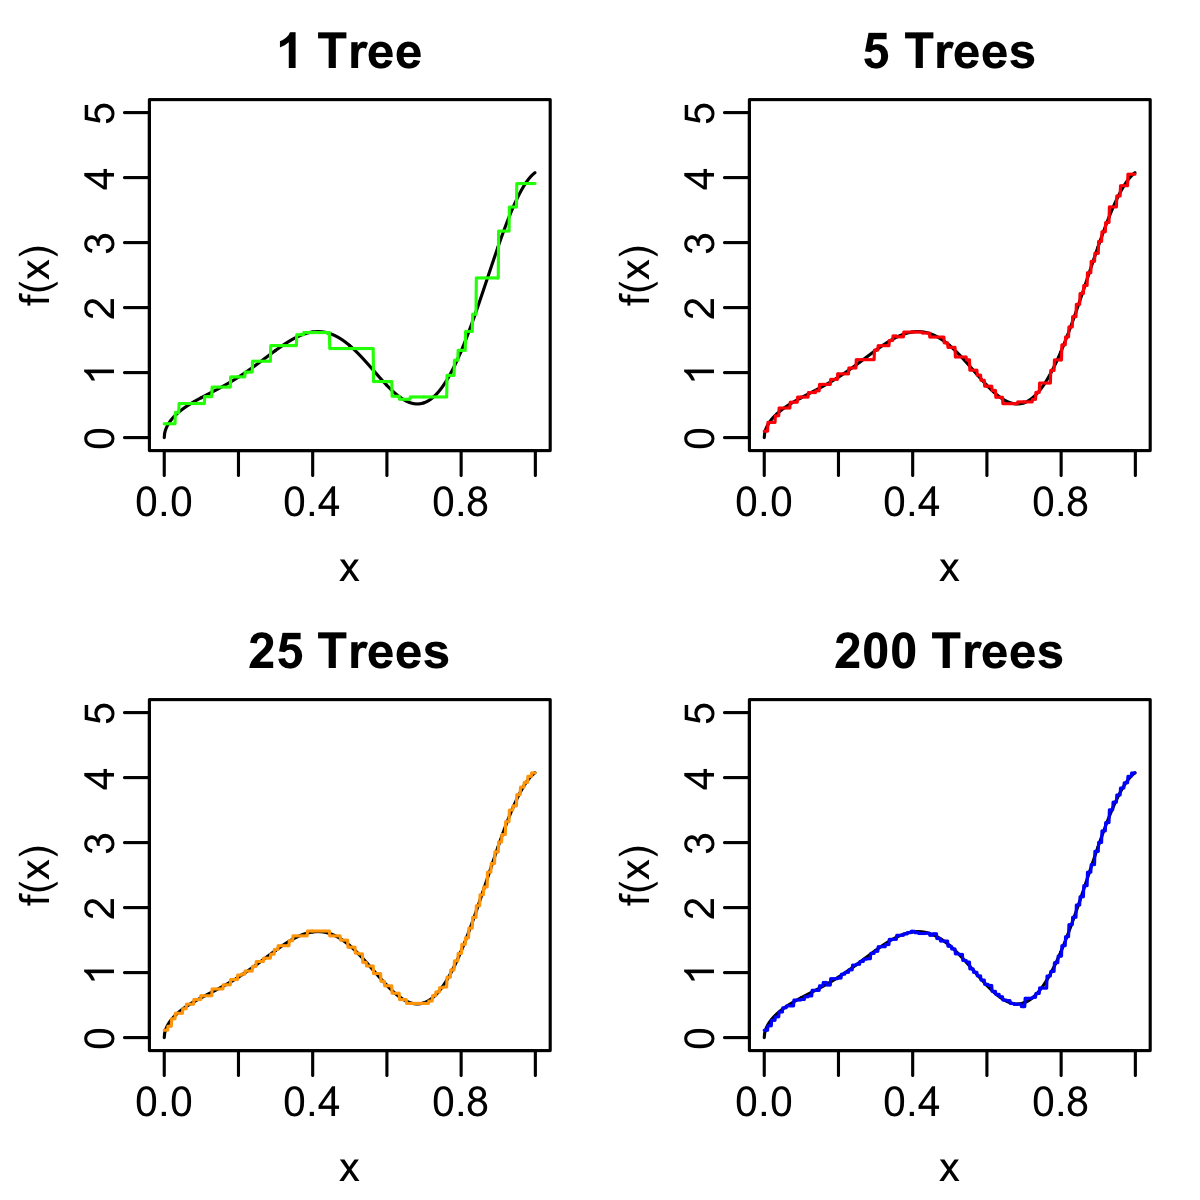
\includegraphics[width = 0.9\textwidth]{figures/sum_of_trees_smooth}
\end{column}
\visible<2->{
\begin{column}{0.3\textwidth}
\centering
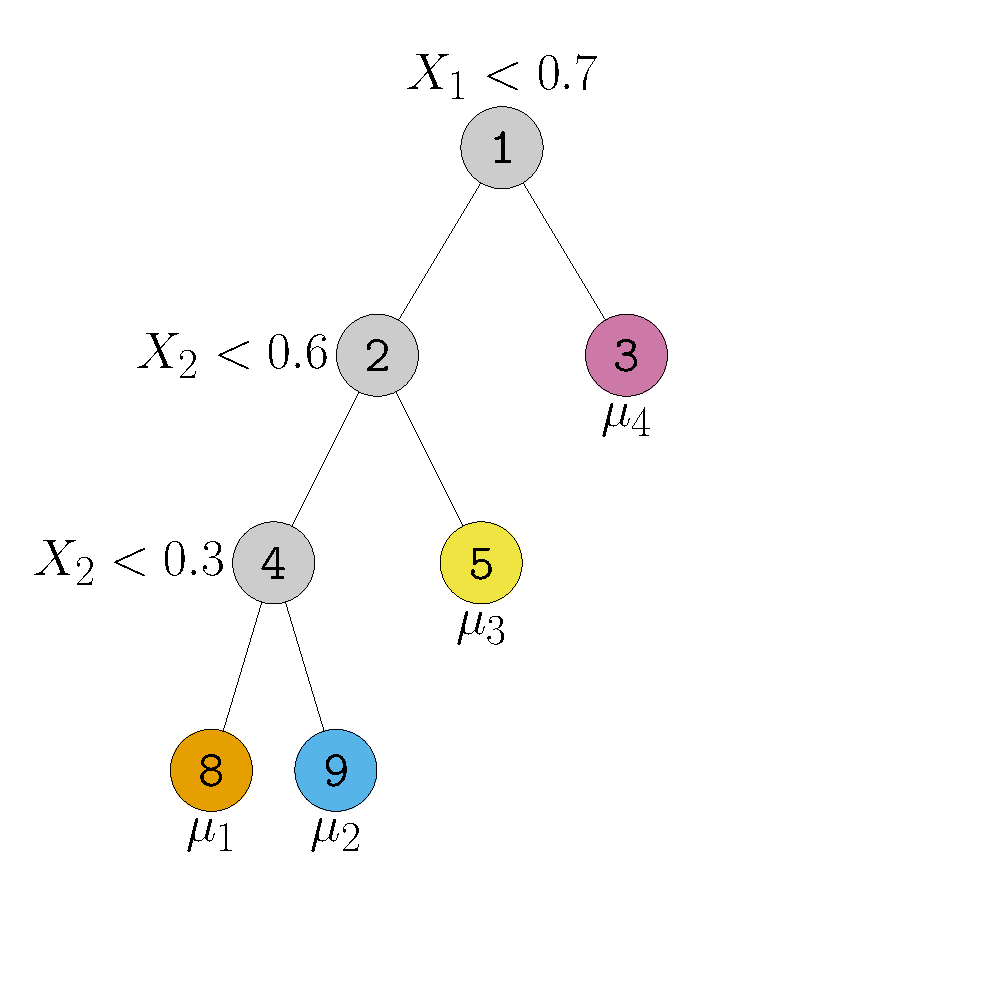
\includegraphics[width = \textwidth]{figures/old_decision_rule}
\end{column}
\begin{column}{0.3\textwidth}
\centering
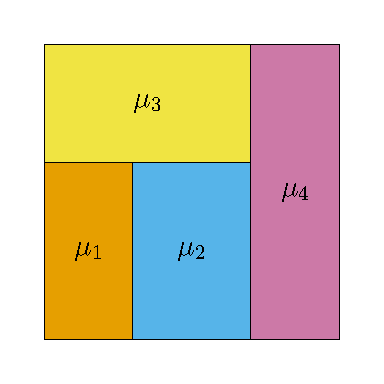
\includegraphics[width = \textwidth]{figures/old_partition}
\end{column}
}
\end{columns}

\begin{itemize}
\item{Step functions are universal function approximators!}
\visible<2->{
\item{Step functions can be represented as binary regression trees}
}
\visible<3->{
\item[\Walley]{Often need very deep tree to appx complicated $f$ well}
}
\end{itemize}

\end{frame}

\begin{frame}{Sums of trees}

\begin{center}
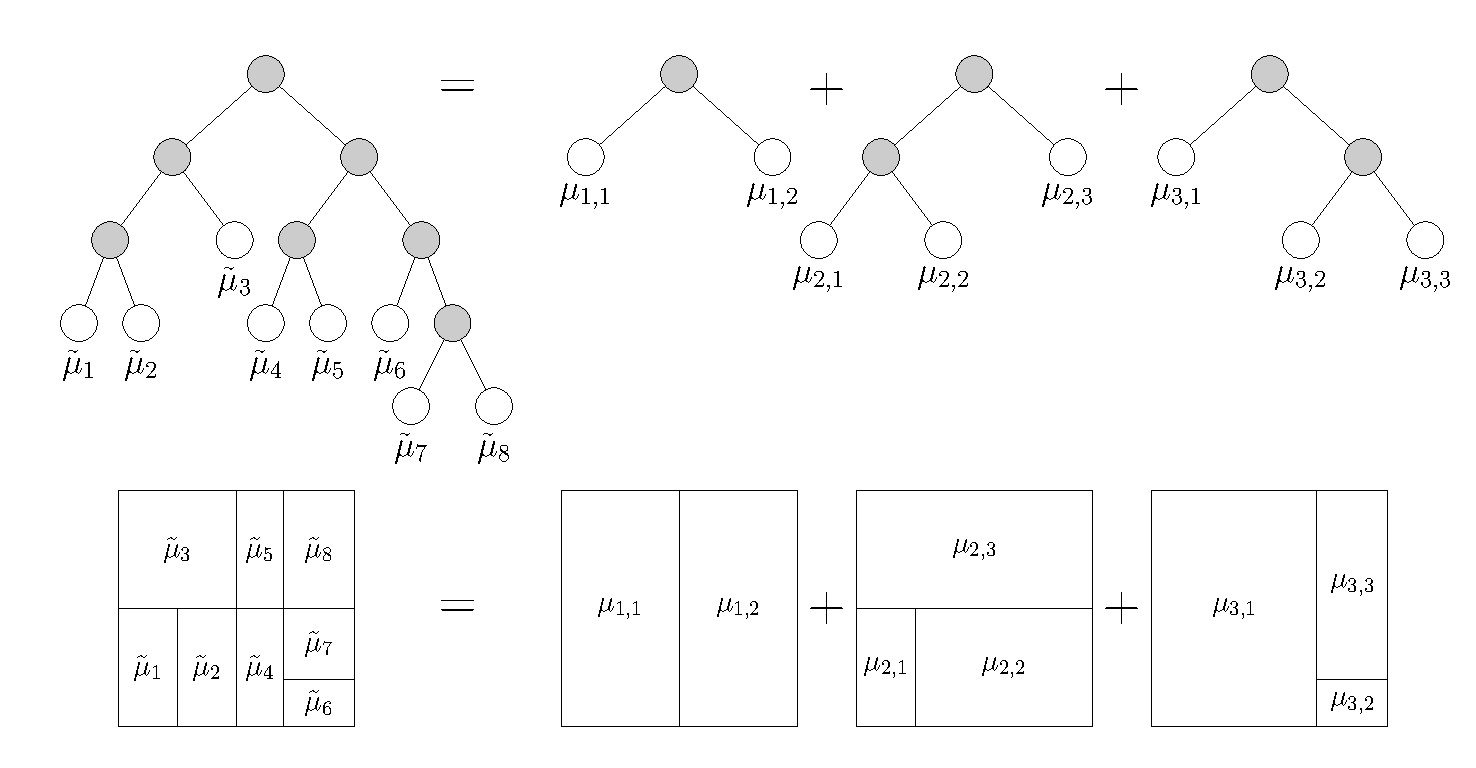
\includegraphics[width = 0.5\textwidth]{figures/sum_of_trees}
\end{center}

\begin{itemize}
\item{Sum of step functions is just another step function!}
\item{Sums of regression trees is a more complicated regression tree!}
\item[\Smiley]{Averaging/ensembling introduces certain degree of smoothness}

\end{itemize}

\end{frame}

\begin{frame}{Digression: Pointillism}


\begin{center}
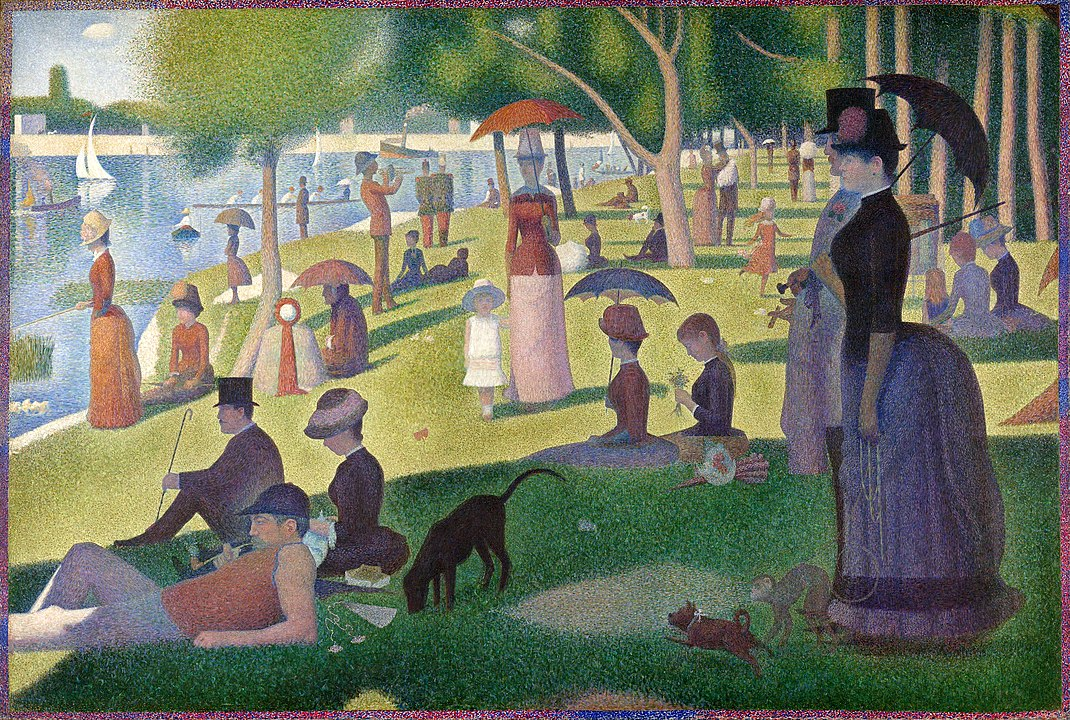
\includegraphics[width = 0.75\textwidth]{figures/seurat_full}
\end{center}

\textit{A Sunday afternoon on the island of La Grande Jatte}, Georges Seurat \href{https://commons.wikimedia.org/wiki/File:A_Sunday_on_La_Grande_Jatte,_Georges_Seurat,_1884.jpg}{Source}

\end{frame}

\section{Introducing BART}
\begin{frame}[noframenumbering]
\tableofcontents[currentsection]
\end{frame}

\begin{frame}{Bayesian Additive Regression Trees}
\begin{itemize}
\item{Regression: $y_{n} = f(\bx_{n}) + \sigma \varepsilon_{n}; \varepsilon_{n} \sim \normaldist{0}{1}$ \& $\bx_{n} \in [0,1]^{p}$}
\item{Main idea: approximate $f(\bx)$ with sum of $M$ regression trees} 
\item{Prior encourages trees to be ``weak learners''}
\item{Gibbs sampler: update each tree conditionally on fit of all others}

\end{itemize}
% sum of trees figure

\begin{columns}

\begin{column}{0.35\textwidth}
\centering
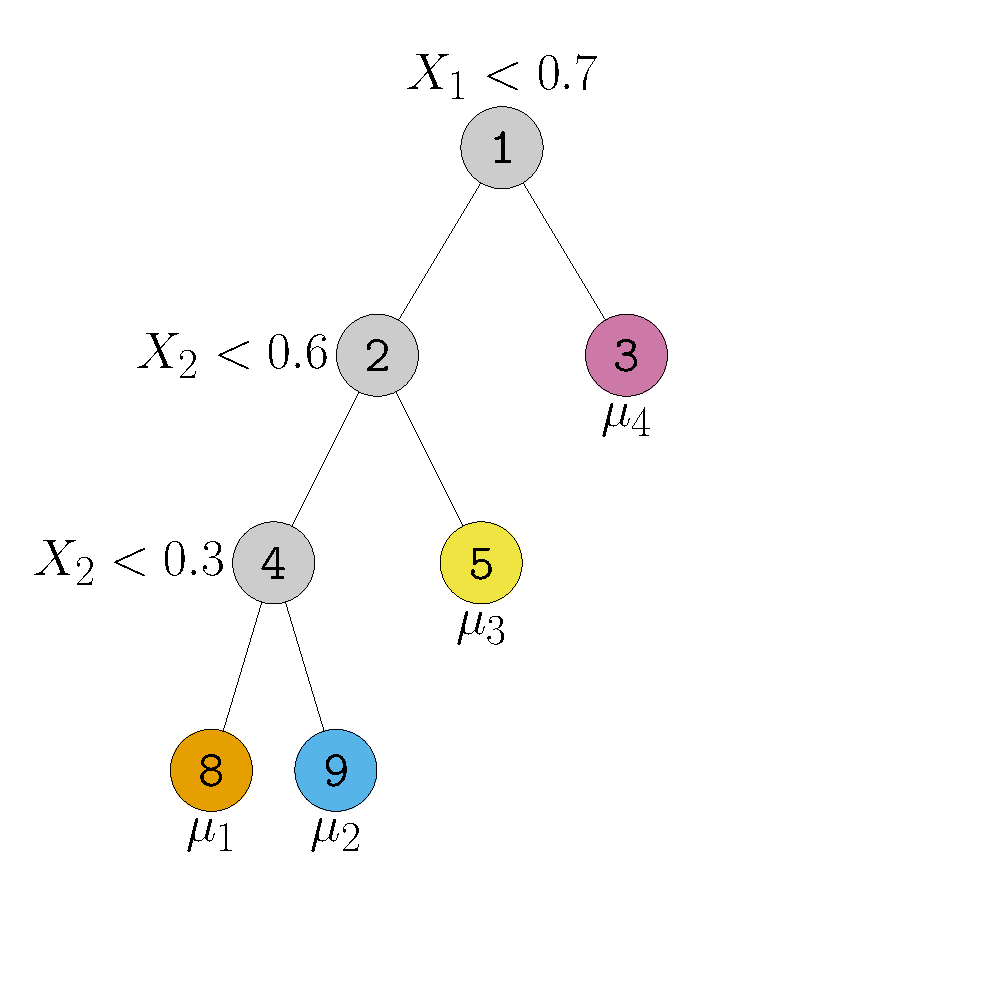
\includegraphics[width = 0.9\textwidth]{figures/old_decision_rule}
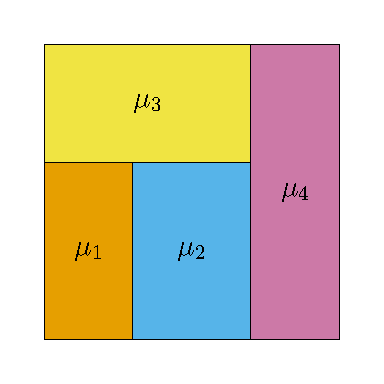
\includegraphics[width = 0.4\textwidth]{figures/old_partition}
\end{column}
\begin{column}{0.6\textwidth}
\centering
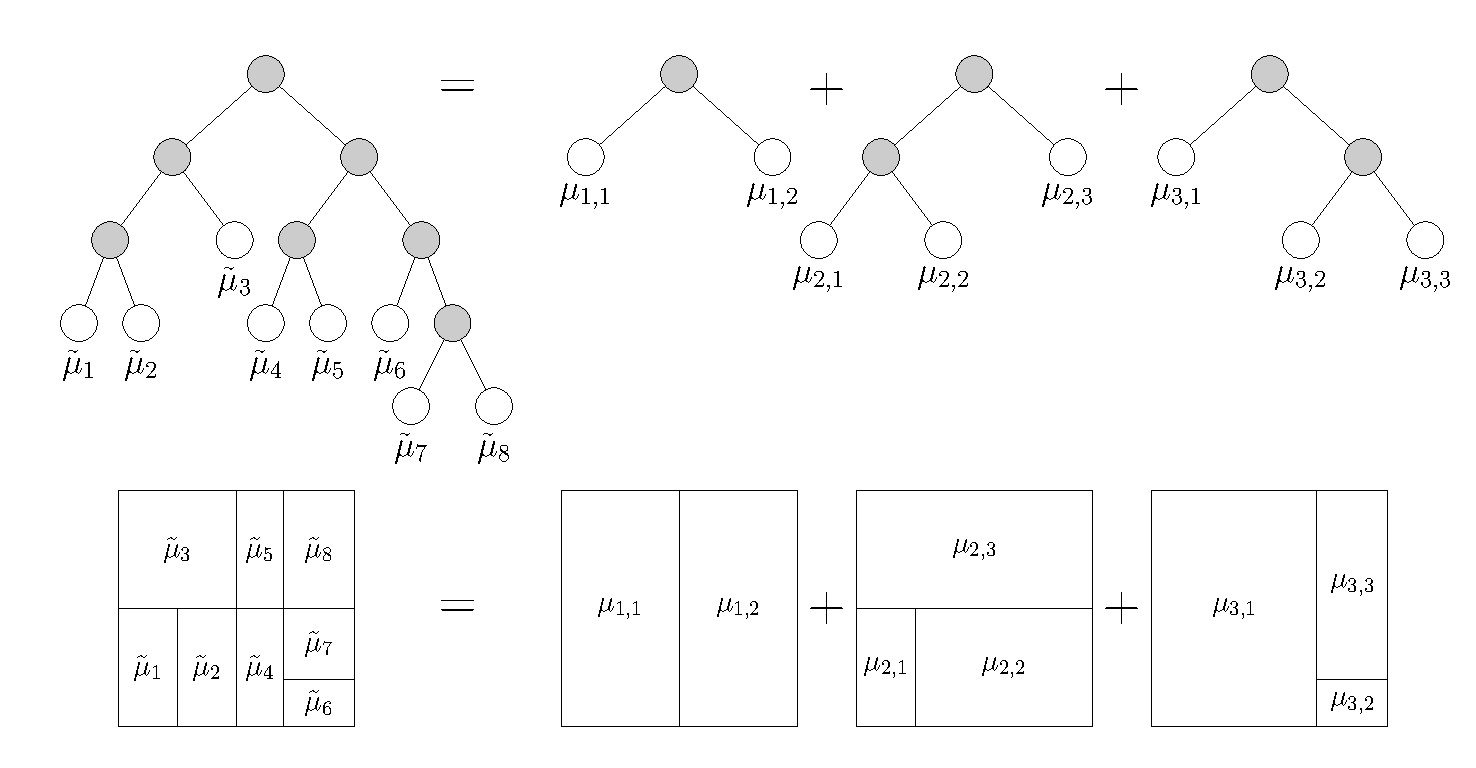
\includegraphics[width = \textwidth]{figures/sum_of_trees}
\end{column}

\end{columns}
\end{frame}

\begin{frame}{Posterior computation \& implementation}

\begin{itemize}
\item{Metropolis-within-Gibbs: update each tree sequentially fixing others}
\begin{itemize}
\item{Update decision tree with MH (randomly grow or prune tree)}
\item{Update leaf parameters / tree outputs conditional on tree}
\end{itemize}
\item{No optimization involved!!}
%\item{When growing tree, convenient to draw new decision rule from prior}
%\begin{itemize}
%\item[\Smiley]{Cancellation in MH ratio $\Rightarrow$ fast tree updates}
%\item[\Smiley]{No optimization needed}
%\end{itemize}
\end{itemize}

\begin{center}
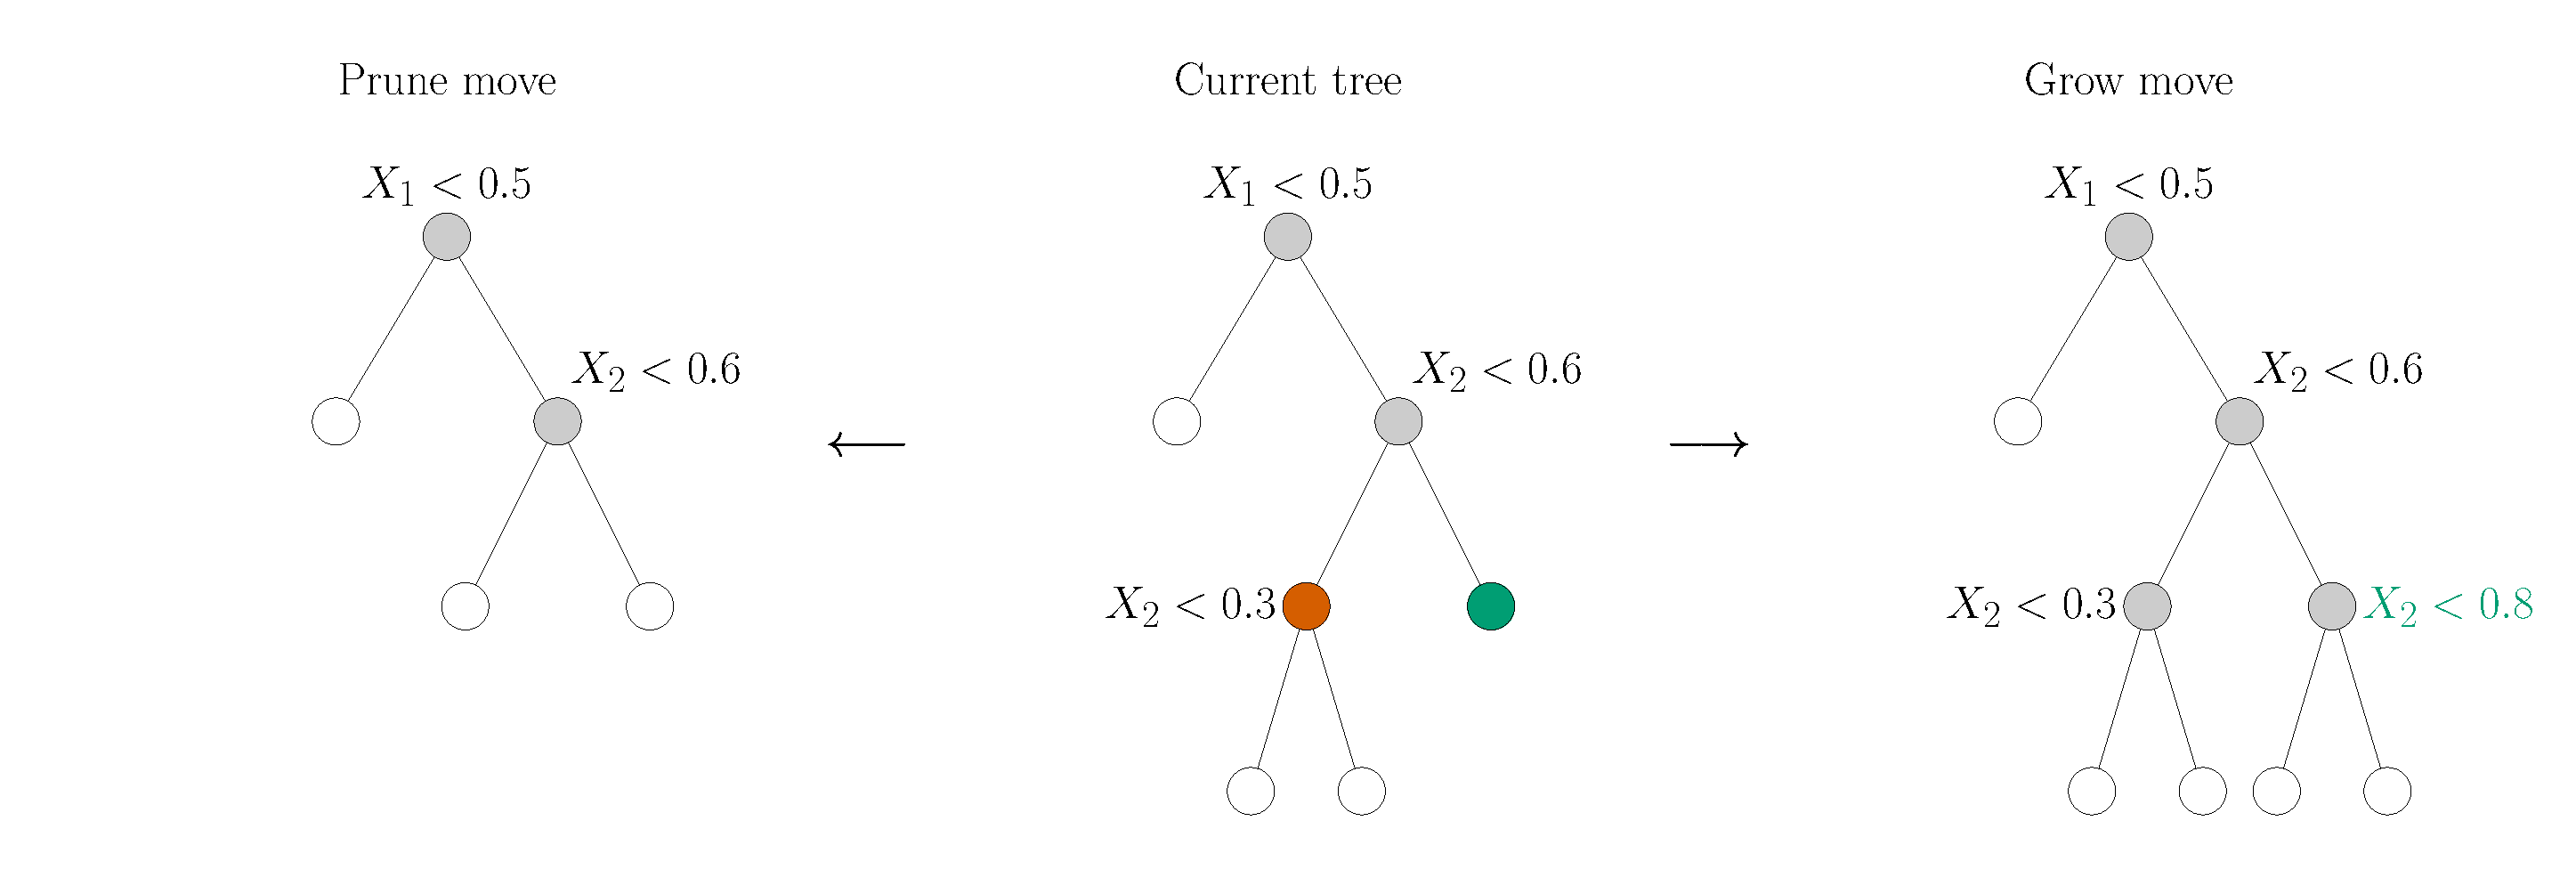
\includegraphics[width = \textwidth]{figures/grow_prune}
\end{center}

\end{frame}


\section{BART in practice}
\begin{frame}[noframenumbering]{Outline}
\tableofcontents[currentsection]
\end{frame}

\begin{frame}{Several implementations}

\begin{itemize}
\item{\textbf{BART}: \href{https://cran.r-project.org/web/packages/BART/index.html}{Sparapani, Spanbauer, \& McCulloch (2021)}}
\begin{itemize}
%\item{Maintained by original authors + their collaborators}
\item{Support for many extensions (e.g., classification, survival)}
\item{Based on efficient C++ regression tree class \& sampler}
\end{itemize}

\item{\textbf{dbarts}: \href{https://cran.r-project.org/web/packages/dbarts/index.html}{Dorie (2020)}}
\begin{itemize}
\item{Makes it easy to include a sum-of-trees component in a larger model}
\item{E.g. $y_{i} = \bx_{i}^{\top}\beta + f(\bx_{i}) + \sigma \epsilon_{i}$}
\end{itemize}

\item{\textbf{flexBART}: available at \href{https://github.com/skdeshpande91/flexBART}{(GitHub repo)}}
\begin{itemize}
\item{Flexibly handle categorical predictors and observations on networks}
\item{Much faster than \textbf{BART}}
\item{Still under active development}
\end{itemize}

\item{\textbf{bartMachine}: \href{https://cran.r-project.org/web/packages/bartMachine/index.html}{Kapelner \& Bleich (2014)}}
\begin{itemize}
\item{Core fitting written in Java}
\item[\Annoey]{Non-trivial overhead in installing \& setting up system}
\end{itemize}

\item{\textbf{PyMC-BART}: \href{https://www.pymc.io/projects/bart}{From the PyMC team}}
\begin{itemize}
\item{Uses sequential Monte Carlo \& is rather different than the above}
\end{itemize}

\end{itemize}

\end{frame}


\section{Parting Thoughts}
\begin{frame}[noframenumbering]{Outline}
\tableofcontents[currentsection]
\end{frame}

\begin{frame}{Variable importance \& selection}

\begin{itemize}
\item{Variable importance in treed models is still area of on-going research}
\item{For BART, counting \# decision rules using $X_{j}$ \textbf{\textcolor{BadgerRed}{not recommended}}}

\visible<2->{
\item{Partial dependence plots}
\begin{itemize}
\item{$\overline{f}_{j}(\textcolor{SkyBlue}{x}) = n^{-1}\sum_{i}{f(x_{i,1}, \ldots, x_{i,j-1}, \textcolor{SkyBlue}{x}, x_{i,j+1}, \ldots, x_{i,p})}$}
\item{Implemented in \texttt{dbarts::pdbart} and easy to do by hand}
\end{itemize}
}
\visible<3->{
\item{\href{https://www.tandfonline.com/doi/full/10.1080/01621459.2016.1264957}{Linero (2018)} modifies BART so that}
\begin{itemize}
\item{Split on $X_{j}$ with prob. $\theta_{j}$ (in prior \& in MH transition)}
\item{$\boldsymbol{\theta}$ given a sparsity-inducing Dirichlet prior}
\item{Adaptation: more accepted splits on $X_{j} \Rightarrow$ more proposed splits on $X_{j}$}
\item{Select $X_{j}$ if more than 50\% of ensembles involve a split on $X_{j}$}
\end{itemize}
}
\end{itemize}
\end{frame}

\begin{frame}{BART extensions}

\begin{itemize}
\item{Classification: probit w/ \href{https://www.tandfonline.com/doi/abs/10.1080/01621459.1993.10476321}{Albert \& Chib (1993)} data augmentation}
\item{Survival models: \href{https://onlinelibrary.wiley.com/doi/abs/10.1002/sim.6893}{Sparapani et al. (2016)}}
\item{Log-linear models: \href{https://arxiv.org/abs/1701.01503}{Murray (2019)}}
\item{Heteroscedasticity: \href{https://www.tandfonline.com/doi/abs/10.1080/10618600.2019.1677243?journalCode=ucgs20}{Pratola et al. (2020)}}
\begin{itemize}
\item{$y_{n} = f(\bx_{n}) + \sigma(\bx_{n})\varepsilon_{n}$, write $\log{(\sigma^{2}(\bx))}$ as a sum-of-trees! }
\end{itemize}
\item{Monotonic BART: \href{https://arxiv.org/abs/1612.01619}{Chipman et al. (2019)}}
\item{Estimating smooth functions}
\begin{itemize}
\item{\href{https://projecteuclid.org/journals/annals-of-applied-statistics/volume-14/issue-1/BART-with-targeted-smoothing--An-analysis-of-patient-specific/10.1214/19-AOAS1268.short}{Starling et al. (2020)}: jumps $\mu_{\ell}$ are Gaussian processes}
\end{itemize}
\item{Varying coefficient models: \href{https://arxiv.org/abs/2003.06416}{D. et al. (2020+)}}
\begin{itemize}
\item{$Y = \beta_{0}(Z) + \beta_{1}(Z)X_{1} + \cdots + \beta_{p}(Z)X_{p} + \sigma\epsilon$}
\item{E.g. time \& demographic varying mediation effects}
\end{itemize}
\item{Causal inference: \href{https://www.tandfonline.com/doi/abs/10.1198/jcgs.2010.08162}{Hill (2011)} \& \href{https://projecteuclid.org/journals/bayesian-analysis/volume-15/issue-3/Bayesian-Regression-Tree-Models-for-Causal-Inference--Regularization-Confounding/10.1214/19-BA1195.full}{Hahn et al (2020)}}
\end{itemize}

\end{frame}

\begin{frame}{Concluding remarks}

\begin{itemize}
\item{BART: approximate $f$ with sum of regression trees}
\item{Avoids pre-specification of functional form of $f(\bx) = \E[Y \mid X = \bx]$}
\item{Excellent performance off-the-shelf}
\item{Lots still in development ... get in touch!}
\end{itemize}

\visible<2->{
\vskip 0.5cm
\makebox[0.95\paperwidth]{
\hfill
\LARGE{Thanks, y'all!}
\hfill
}

\vskip 0.125cm
\makebox[0.95\paperwidth]{
Email: \texttt{\textcolor{BadgerRed}{sameer.deshpande@wisc.edu}} \hfill
}
\makebox[0.95\paperwidth]{
Website: \url{https://skdeshpande91.github.io} \hfill
}
\makebox[0.95\paperwidth]{
Twitter: @skdeshpande91 \hfill
}
}
\end{frame}




\appendix
\begin{frame}[noframenumbering]{A prior over regression trees}

\begin{columns}
\centering
\begin{column}{0.33\textwidth}
\centering
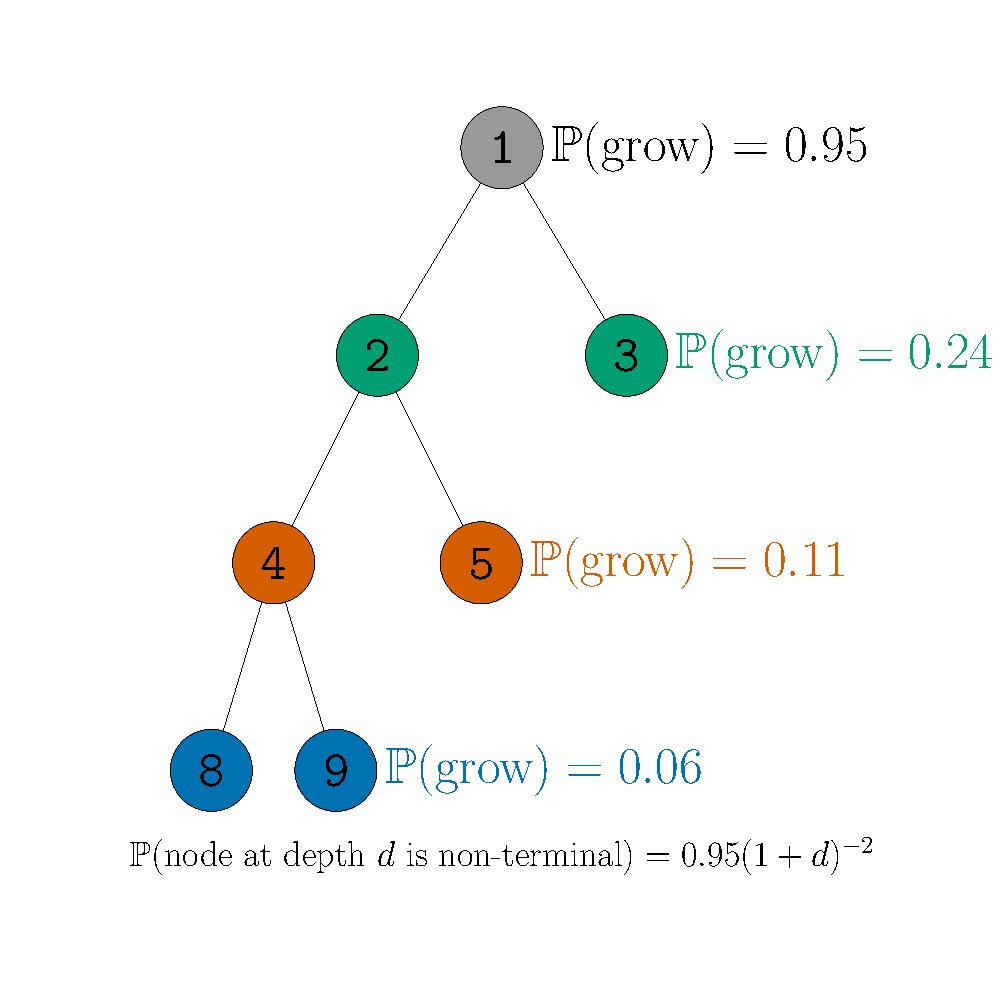
\includegraphics[width = \textwidth]{figures/branching_process}
\end{column}
\visible<2->{
\begin{column}{0.33\textwidth}
\centering
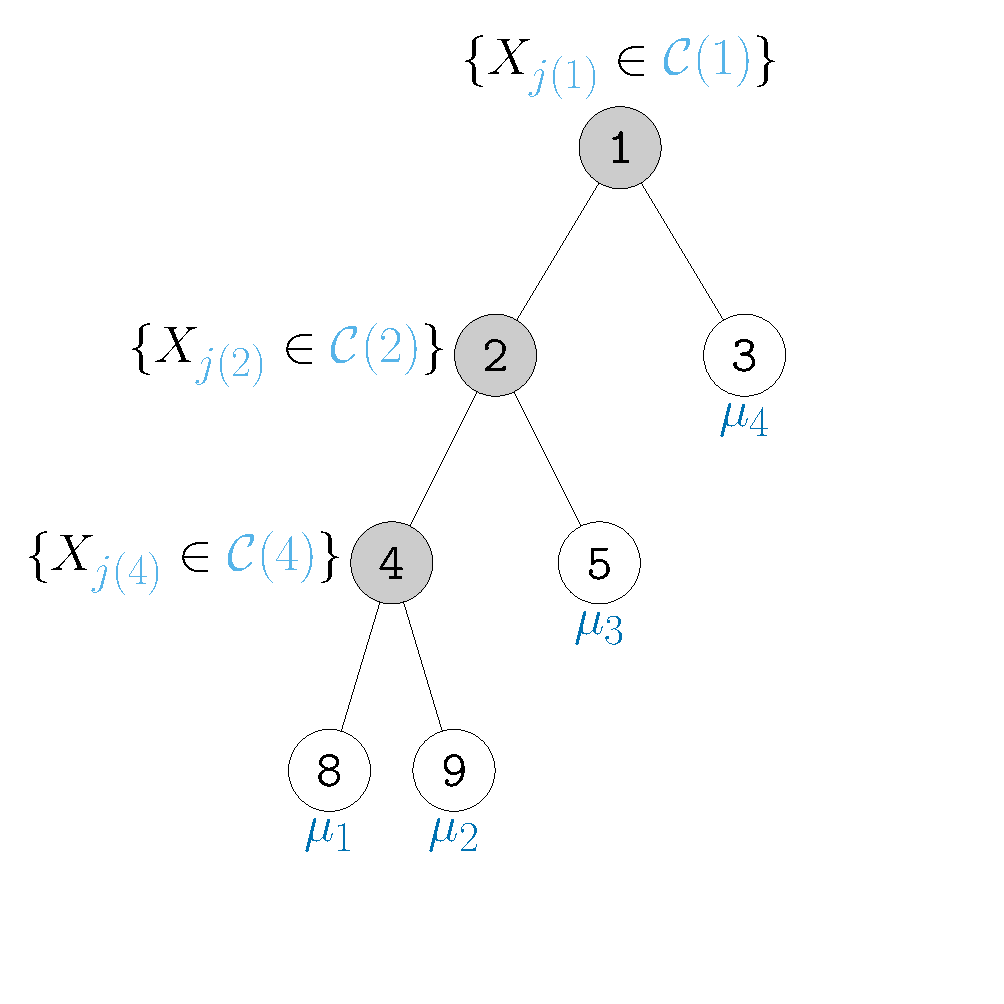
\includegraphics[width = \textwidth]{figures/regression_tree_new}
\end{column}
}
\visible<3->{
\begin{column}{0.33\textwidth}
\centering
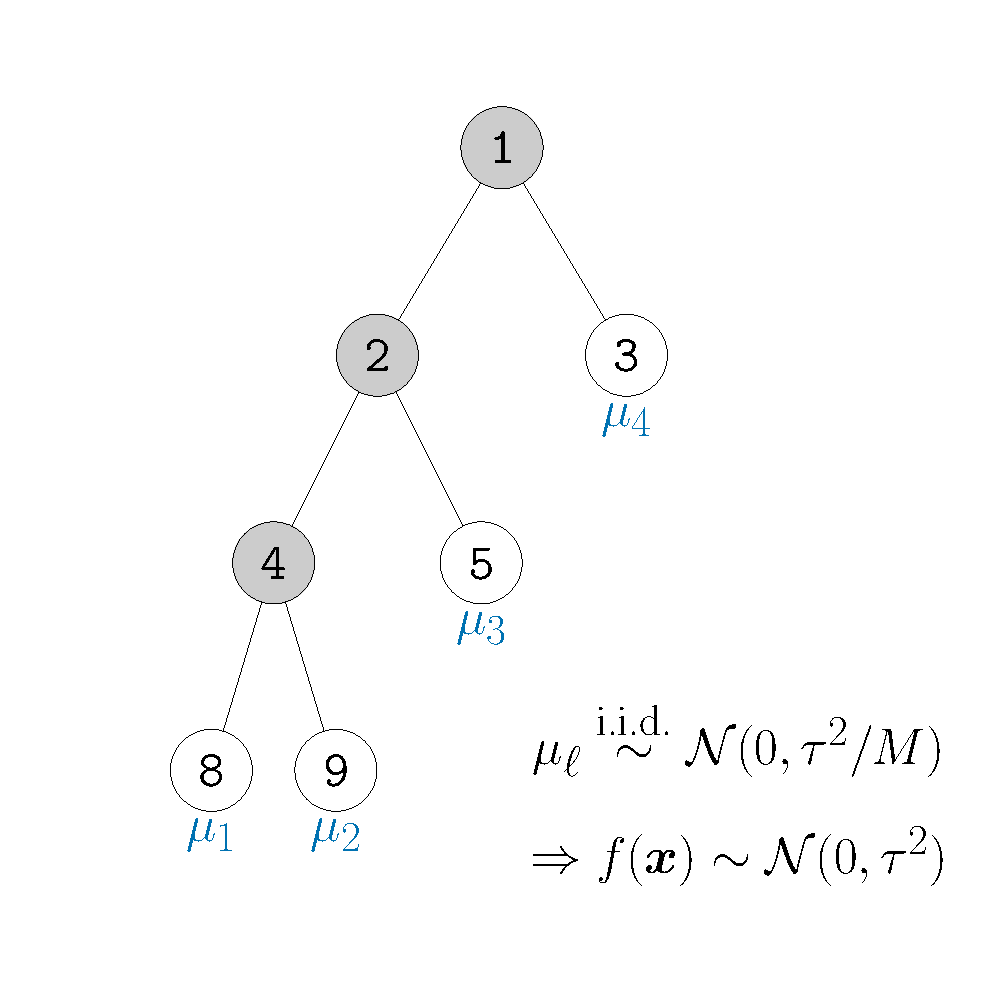
\includegraphics[width = \textwidth]{figures/jumps}
\end{column}
}
\end{columns}
\begin{itemize}
\visible<1->{
\item{Branching process prior on graphical structure}
\item{Overwhelming prior prob. that tree depth $< 5$}
}
\visible<2->{
\item{Decision rule $\{X_{j} \in \mathcal{C}\}$}
\begin{itemize}
\item{$X_{j}$ continuous: $\mathcal{C}$ is an interval $[0,c)$}
\item{$X_{j}$ categorical: $\mathcal{C}$ is a discrete subset of $X_{j}$'s levels}
\end{itemize}
}
\visible<3->{
\item{Leaf outputs $\textcolor{myColor6}{\mu_{\ell}} \stackrel{\text{i.i.d.}}{\sim} \mathcal{N}(0, \tau^{2}/M)$}
}
\end{itemize}

\end{frame}

\begin{frame}[noframenumbering]{Decision rule prior}

\begin{columns}

\begin{column}{0.6\textwidth}
\begin{enumerate}
\item{Draw $j \sim \text{Multinomial}(\theta_{1}, \ldots, \theta_{p})$ where $\theta_{j} = \P(\text{split on $X_{j}$})$}
\item{Compute set of all available values $\mathcal{A}_{j}$}
\begin{itemize}
\item{$\mathcal{A}_{j}$ determined by rules at ancestors}
\item{$X_{j}$ continuous $\rightarrow$ $\mathcal{A}$ is an interval}
\item{$X_{j}$ categorical $\rightarrow$ $\mathcal{A}$ is discrete set}
\end{itemize}
\item{Draw random subset $\mathcal{C}$ from $\mathcal{A}_{j}$}
\begin{itemize}
\item{$X_{j}$ ccontinuous: draw $c \sim \mathcal{U}(\mathcal{A}_{j})$ and set $\mathcal{C} = [0,c)$}
\item{$X_{j}$ categorical: assign elements of $\mathcal{A}_{j}$ to $\mathcal{C}$ with probability 0.5}
\end{itemize}
\end{enumerate}

\end{column}
\begin{column}{0.4\textwidth}
\centering
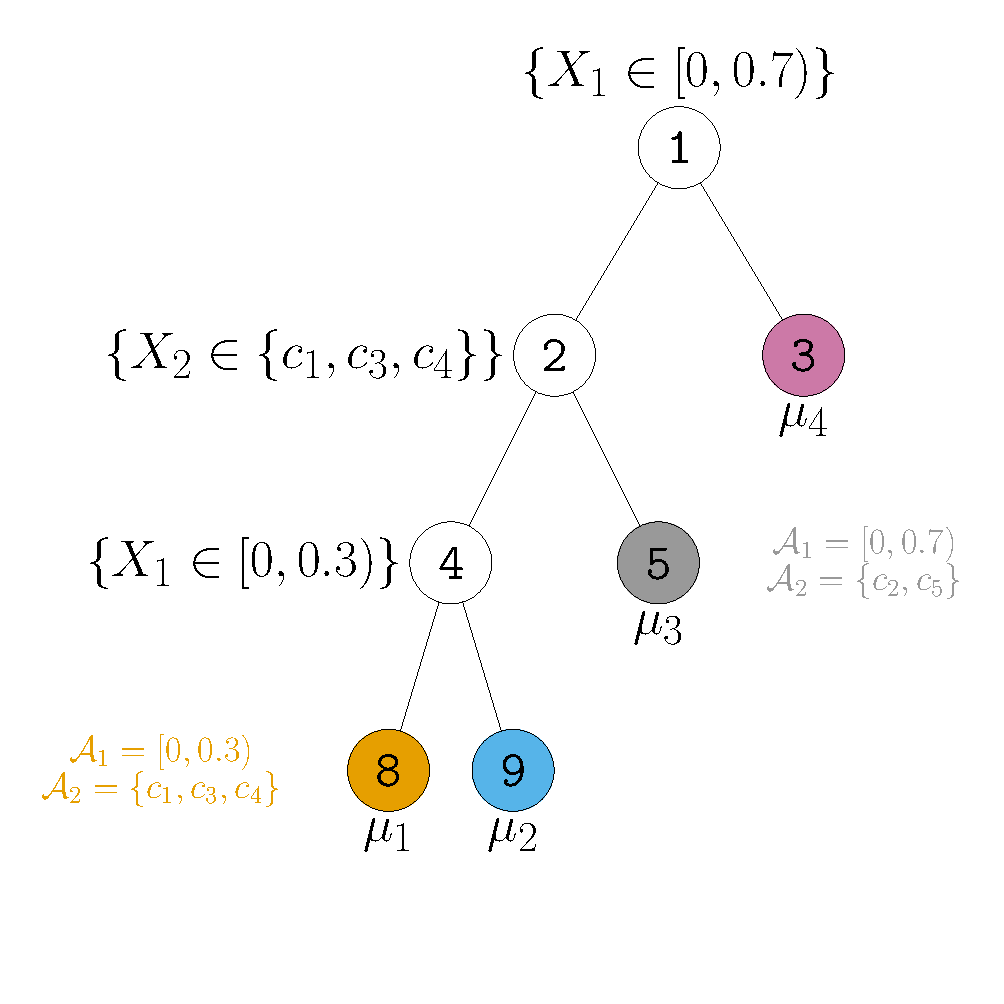
\includegraphics[width = \textwidth]{figures/decision_rule_new}
\end{column}

\end{columns}
\end{frame}






\end{document}